\documentclass[bachelor, och, labwork]{shiza}
% параметр - тип обучения - одно из значений:
%    spec     - специальность
%    bachelor - бакалавриат (по умолчанию)
%    master   - магистратура
% параметр - форма обучения - одно из значений:
%    och   - очное (по умолчанию)
%    zaoch - заочное
% параметр - тип работы - одно из значений:
%    referat    - реферат
%    coursework - курсовая работа (по умолчанию)
%    diploma    - дипломная работа
%    pract      - отчет по практике
% параметр - включение шрифта
%    times    - включение шрифта Times New Roman (если установлен)
%               по умолчанию выключен
\usepackage{subfigure}
\usepackage{tikz,pgfplots}
\pgfplotsset{compat=1.5}
\usepackage{float}

%\usepackage{titlesec}
\setcounter{secnumdepth}{4}
%\titleformat{\paragraph}
%{\normalfont\normalsize}{\theparagraph}{1em}{}
%\titlespacing*{\paragraph}
%{35.5pt}{3.25ex plus 1ex minus .2ex}{1.5ex plus .2ex}

\titleformat{\paragraph}[block]
{\hspace{1.25cm}\normalfont}
{\theparagraph}{1ex}{}
\titlespacing{\paragraph}
{0cm}{2ex plus 1ex minus .2ex}{.4ex plus.2ex}

% --------------------------------------------------------------------------%


\usepackage[T2A]{fontenc}
\usepackage[utf8]{inputenc}
\usepackage{graphicx}
\graphicspath{ {./images/} }
\usepackage{tempora}

\usepackage[sort,compress]{cite}
\usepackage{amsmath}
\usepackage{amssymb}
\usepackage{amsthm}
\usepackage{fancyvrb}
\usepackage{listings}
\usepackage{listingsutf8}
\usepackage{longtable}
\usepackage{array}
\usepackage[english,russian]{babel}

\usepackage[colorlinks=false]{hyperref}
\usepackage{url}

\usepackage{underscore}
\usepackage{setspace}
\usepackage{indentfirst} 
\usepackage{mathtools}
\usepackage{amsfonts}
\usepackage{enumitem}
\usepackage{tikz}
\usepackage{minted}


\newcommand{\eqdef}{\stackrel {\rm def}{=}}
\newcommand{\specialcell}[2][c]{%
\begin{tabular}[#1]{@{}c@{}}#2\end{tabular}}

\renewcommand\theFancyVerbLine{\small\arabic{FancyVerbLine}}

\newtheorem{lem}{Лемма}

\begin{document}

% Кафедра (в родительном падеже)
\chair{теоретических основ компьютерной безопасности и криптографии}

% Тема работы
\title{Сортировка с помощью прямого включения}

% Курс
\course{3}

% Группа
\group{331}

% Факультет (в родительном падеже) (по умолчанию "факультета КНиИТ")
\department{факультета КНиИТ}

% Специальность/направление код - наименование
%\napravlenie{09.03.04 "--- Программная инженерия}
%\napravlenie{010500 "--- Математическое обеспечение и администрирование информационных систем}
%\napravlenie{230100 "--- Информатика и вычислительная техника}
%\napravlenie{231000 "--- Программная инженерия}
\napravlenie{100501 "--- Компьютерная безопасность}

% Для студентки. Для работы студента следующая команда не нужна.
% \studenttitle{Студентки}

% Фамилия, имя, отчество в родительном падеже
\author{Токарева Никиты Сергеевича}

% Заведующий кафедрой
% \chtitle{} % степень, звание
% \chname{}

%Научный руководитель (для реферата преподаватель проверяющий работу)
\satitle{доцент} %должность, степень, звание
\saname{А. Н. Гамова}

% Руководитель практики от организации (только для практики,
% для остальных типов работ не используется)
% \patitle{к.ф.-м.н.}
% \paname{С.~В.~Миронов}

% Семестр (только для практики, для остальных
% типов работ не используется)
%\term{8}

% Наименование практики (только для практики, для остальных
% типов работ не используется)
%\practtype{преддипломная}

% Продолжительность практики (количество недель) (только для практики,
% для остальных типов работ не используется)
%\duration{4}

% Даты начала и окончания практики (только для практики, для остальных
% типов работ не используется)
%\practStart{30.04.2019}
%\practFinish{27.05.2019}

% Год выполнения отчета
\date{2022}

\maketitle

% Включение нумерации рисунков, формул и таблиц по разделам
% (по умолчанию - нумерация сквозная)
% (допускается оба вида нумерации)
% \secNumbering

%-------------------------------------------------------------------------------------------

\tableofcontents


\section{Описание алгоритма}

  Пусть имеется последовательность элементов $a_0, a_1, ..., a_{n-1}$. Эту последовательность мысленно можно
  разделить на уже упорядоченную последовательность $a_0, a_1, ..., a_{i-1}$ и на исходную, неупорядоченную,
  $a_i, a_{i+1}, ..., a_{n-1}$. Очевидно, что первоначально упорядоченная последовательность состоит из единственного
  элемента $a_0$. При каждом шаге, начиная с $i=1$ и увеличивая $i$ каждый раз на единицу, из исходной последовательности
  извлекается $i$-й элемент $a_i$, и вставляется в готовую последовательность в нужное место, при необходимости, сдвигая
  элементы готовой последовательности на одну позицию вправо вплоть до $i$-й позиции. Поиск подходящего места осуществляется
  сравнением $a_i$ с элементами $a_j$, где $j=i-1, i-2,...0$, и одовременным обменом местами $a_i$, и $a_j$, если $a_i < a_j$,
  т.е. сдвигом $a_j$ на одну позицию вправо. 
  
  Процесс поиска заканчивается при выполнении одного из условий:
  
  \begin{itemize}
    \item если $a_i \geq a_j$;
    \item если достигнут левый конец готовой последовательности.
  \end{itemize}

  \section{Код программы, реализующий алгоритм}

  Далее представлена реализация сортировки с помощью прямого включения.

  % \lstinputlisting[language=C++]{code/straight_insertion_sort.cpp}

  \inputminted[fontsize=\small]{C++}{code/sort.cpp}

  Далее приведем несколько примеров, подав некоторые случайные числа в качестве входных данных, чтобы проверить корректность, написанного
  кода.

  На рисунке 1 показан ввод 10 случайных чисел.

  \begin{figure}[H]
    \centering
    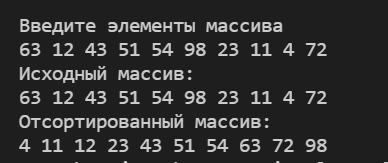
\includegraphics[width=0.8\textwidth]{img/1_1}
    \caption{Ввод последовательности, состоящей из 10 чисел}
  \end{figure}

  На рисунке 2 показан ввод 15 случайных чисел. Отсюда видно, что всё работает корректно.

  \begin{figure}[H]
    \centering
    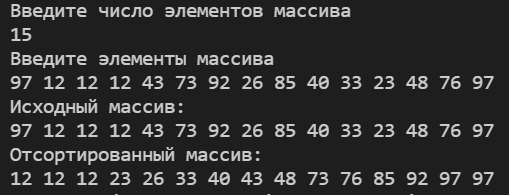
\includegraphics[width=0.8\textwidth]{img/1_2}
    \caption{Ввод последовательности, состоящей из 15 чисел}
  \end{figure}
  
  \section{Анализ алгоритма}

  Количество сравнений элементов ($C_i$) при $i$-м просеивании самое большее равно $i-1$, самое меньшее -- $1$. Если предположить,
  что все перестановки из $n$ элементов равновероятны, то среднее число сравнений -- $i/2$. Число же перессылок (присваиваний
  элементов) $M_i$ равно $C_i+2$. 
  
  Поэтому общее число сравнений:

    $C_{min} = n - 1$
    
    $C_{ave} = (n^2 + n - 2) / 4$

    $C_{max} = (n^2 + n - 4) / 4$

  Общее число перессылок:

    $M_{min} = 3(n - 1)$
    
    $M_{ave} = (n^2 + 9n - 10) / 4$

    $M_{max} = (n^2 + 3n - 4) / 2$

  Минимальные оценки встречаются в случае уже упорядоченной исходной последовательности элементов,
  наихуджие оценки -- когда они первоначально расположены в обратном порядке. В некотором смысле
  сортировка с помощью включений демонстрирует истинно естественное поведение. Ясно, что приведенный
  алгоритм описывает процесс устойчивой сортировке, так как порядок элементов с равными ключами при
  нем остается неизменным.

  % Алгоритм с прямыми включениями можно легко улучшить с учётом того, что готовая последовательность, куда надо вставить новый
  % элемент, уже упорядочена. Тогда место включения ищется методом двоичного (бинарного) поиска. Такой улучшенный алгоритм
  % сортировки называется методом с двоичным включением (методом прямого включения с делением пополам). Однако применение
  % этого алгоритма оправдано только тогда, когда число сортируемых элементов достаточно велико.


  % \subsection{Коды программ, реализующей рассмотренные алгоритмы}

    %     \inputminted[fontsize=\small]{python}{code/lab-1.py}

    % \subsection{Результаты тестирования программ}

        % \begin{figure}[H]
        %     \centering
        %     \includegraphics[width=0.8\textwidth]{pic/pic (1).png}
        %     \caption{}
        % \end{figure}

\conclusion

В данной лабораторной работе была рассмотрена сортировка с помощью прямого включения и был проведен анализ оценки
сложности данного алгоритма. Это послужило созданием её программной реализации, написанной на языке C++. 

\begin{thebibliography}{2}
  \bibitem{1}
  Книга Н. Вирт, "Алгоритмы и структуры данных" / Москва: Мир, 1989 г., Яз. рус.
  \bibitem{2}
  Книга Стивена С. Скиена, "Алгоритмы. Руководство по разработке 2-е издание" / Санкт-Петербург: БХВ-Петербург, 2021 г., Яз. рус.   
\end{thebibliography}

\end{document}
